\setlength{\columnsep}{3pt}
\begin{flushleft}

\begin{itemize}
	\item Buffer is located inside RAM.
	\begin{figure}[h!]
		\centering
		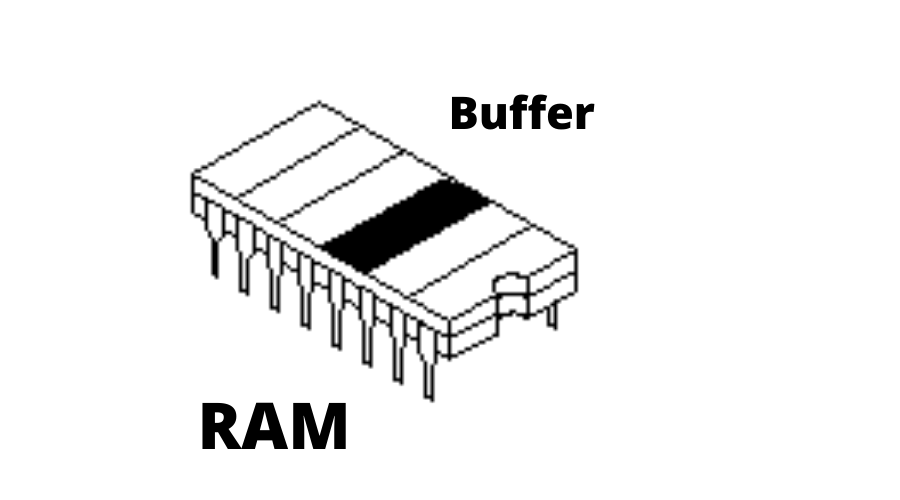
\includegraphics[scale=0.3]{content/chapter12/images/buffer.png}
		\caption{Buffer}
		\label{fig:buffer}
	\end{figure}
	\item Buffer act as a temporary holding area for the CPU to manipulate data before transferring it to a device. 
	\item Buffer usage eg:
	\begin{itemize}
		\item \textbf{Copy operation}: In case of copying data from 1 device to another with device having different speeds, data is stored in buffer.
		\item \textbf{Saving data to HDD}: Word processors write the data first in the buffer, and later updates the file in the disk with the contents of the buffer.
		\item \textbf{Printing}: The documents to be printed is stored in a buffer, and the printer can then access this information at its own pace.
	\end{itemize}
\end{itemize}



\end{flushleft}

\newpage


